\section{Устойчивость по Ляпунову, устойчивость по первому приближению}

	Пусть \( \vec{x}\pares{t} = \begin{pmatrix} x_1\pares{t} \\ \vdots \\ x_n\pares{t} \end{pmatrix} \) -- вектор неизвестных функций, $\vec{f}\pares{\vec{x}} = \begin{pmatrix} f_1 \pares{\vec{x}} \\ \vdots \\ f_n\pares{\vec{x}} \end{pmatrix}$ -- вектор известных функций. Рассматривать будем автономную систему следующего вида:
	\[ \vec{\dot{x}} = \vec{f}\pares{\vec{x}}, ~ t > t_0 \]
	с начальным условием:
	\[ \vec{x}\pares{t_0} = \vec{x}_0. \]
	Положим, что существует точка покоя $\vec{x}\pares{t} = \vec{\vp}_h$ такая, что $f\pares{\vec{\vp}_h} = 0$. Тогда такая точка покоя называется устойчивой, если:
	\[ \forall \varepsilon > 0 ~ \exists \delta > 0: ~ \norm{\vec{x}_0 - \vec{\vp}_h} < \delta \implies \norm{\vec{x}\pares{t} - \vec{\vp}_h} < \varepsilon ~ \forall t \ge t_0. \]
	В случае, если $\lim_{t \to \infty} \norm{\vec{x}\pares{t} - \vec{\vp}_h} = 0$, такая точка покоя называется ассимптотически устойчивой.
	Точкой покоя (или критической точкой) $\vec{\vp}_h$ называется точка, вдоль которой решение уравнения постоянно. Когда решение определяется какими-либо постоянными, такие решения называются стационарными решениями, или решениями равновесия системы.

	Рассмотрим автономную систему:
	\[ \vec{\dot{x}} = \vec{f}\pares{\vec{x}}. \]
	Для определения ее стационарных решений необходимо найти такие постоянные вектора $\vec{x}\pares{t} = \vec{\vp}_k, ~ k \in \overline{1, n}, ~ n \ge 0$, при которых
	\[ f\pares{\vec{\vp}} = \vec{0}. \]
	Находя такие вектора $\vec{\vp}_k$, для исследования устойчивости, можно построить систему первого приближения. На основе собственных значений матрицы, можно судить об устойчивости. Если вещественные части всех собственных значений матрицы первого приближения отрицательны, то система считается устойчивой. Если хотя бы у одного из собственных значений вещественная часть положительна, система считается неустойчивой. В случае, если среди собственных значений есть хотя бы одно значение с нулевой вещественной частью, необходим дополнительный анализ.

	Матрица системы первого приближения представляет собой матрицу Якоби вектор-функции $\vec{f}\pares{\vec{x}}$ в окресности точки покоя $\vec{\vp}_k$.

	\subsection{Примеры}
		Рассмотрим, как ведет себя решение следующего уравнения в геометрическом смысле для любого начального условия:
		\[ y' = \sin{y}, ~ y(0) = C - \const. \]
		Дифференциальное уравнение имеет вид $y' = f(y)$ -- уравнение, зависимое только от искомой функции, или носит название автономного или стационарного. Рассматривать будем в области решений $y \in \bracks{-2\pi, 2\pi}$ Построим график этого уравнения как функции в осях $y'(y)$:
		\begin{figure}[H]
			\centering
			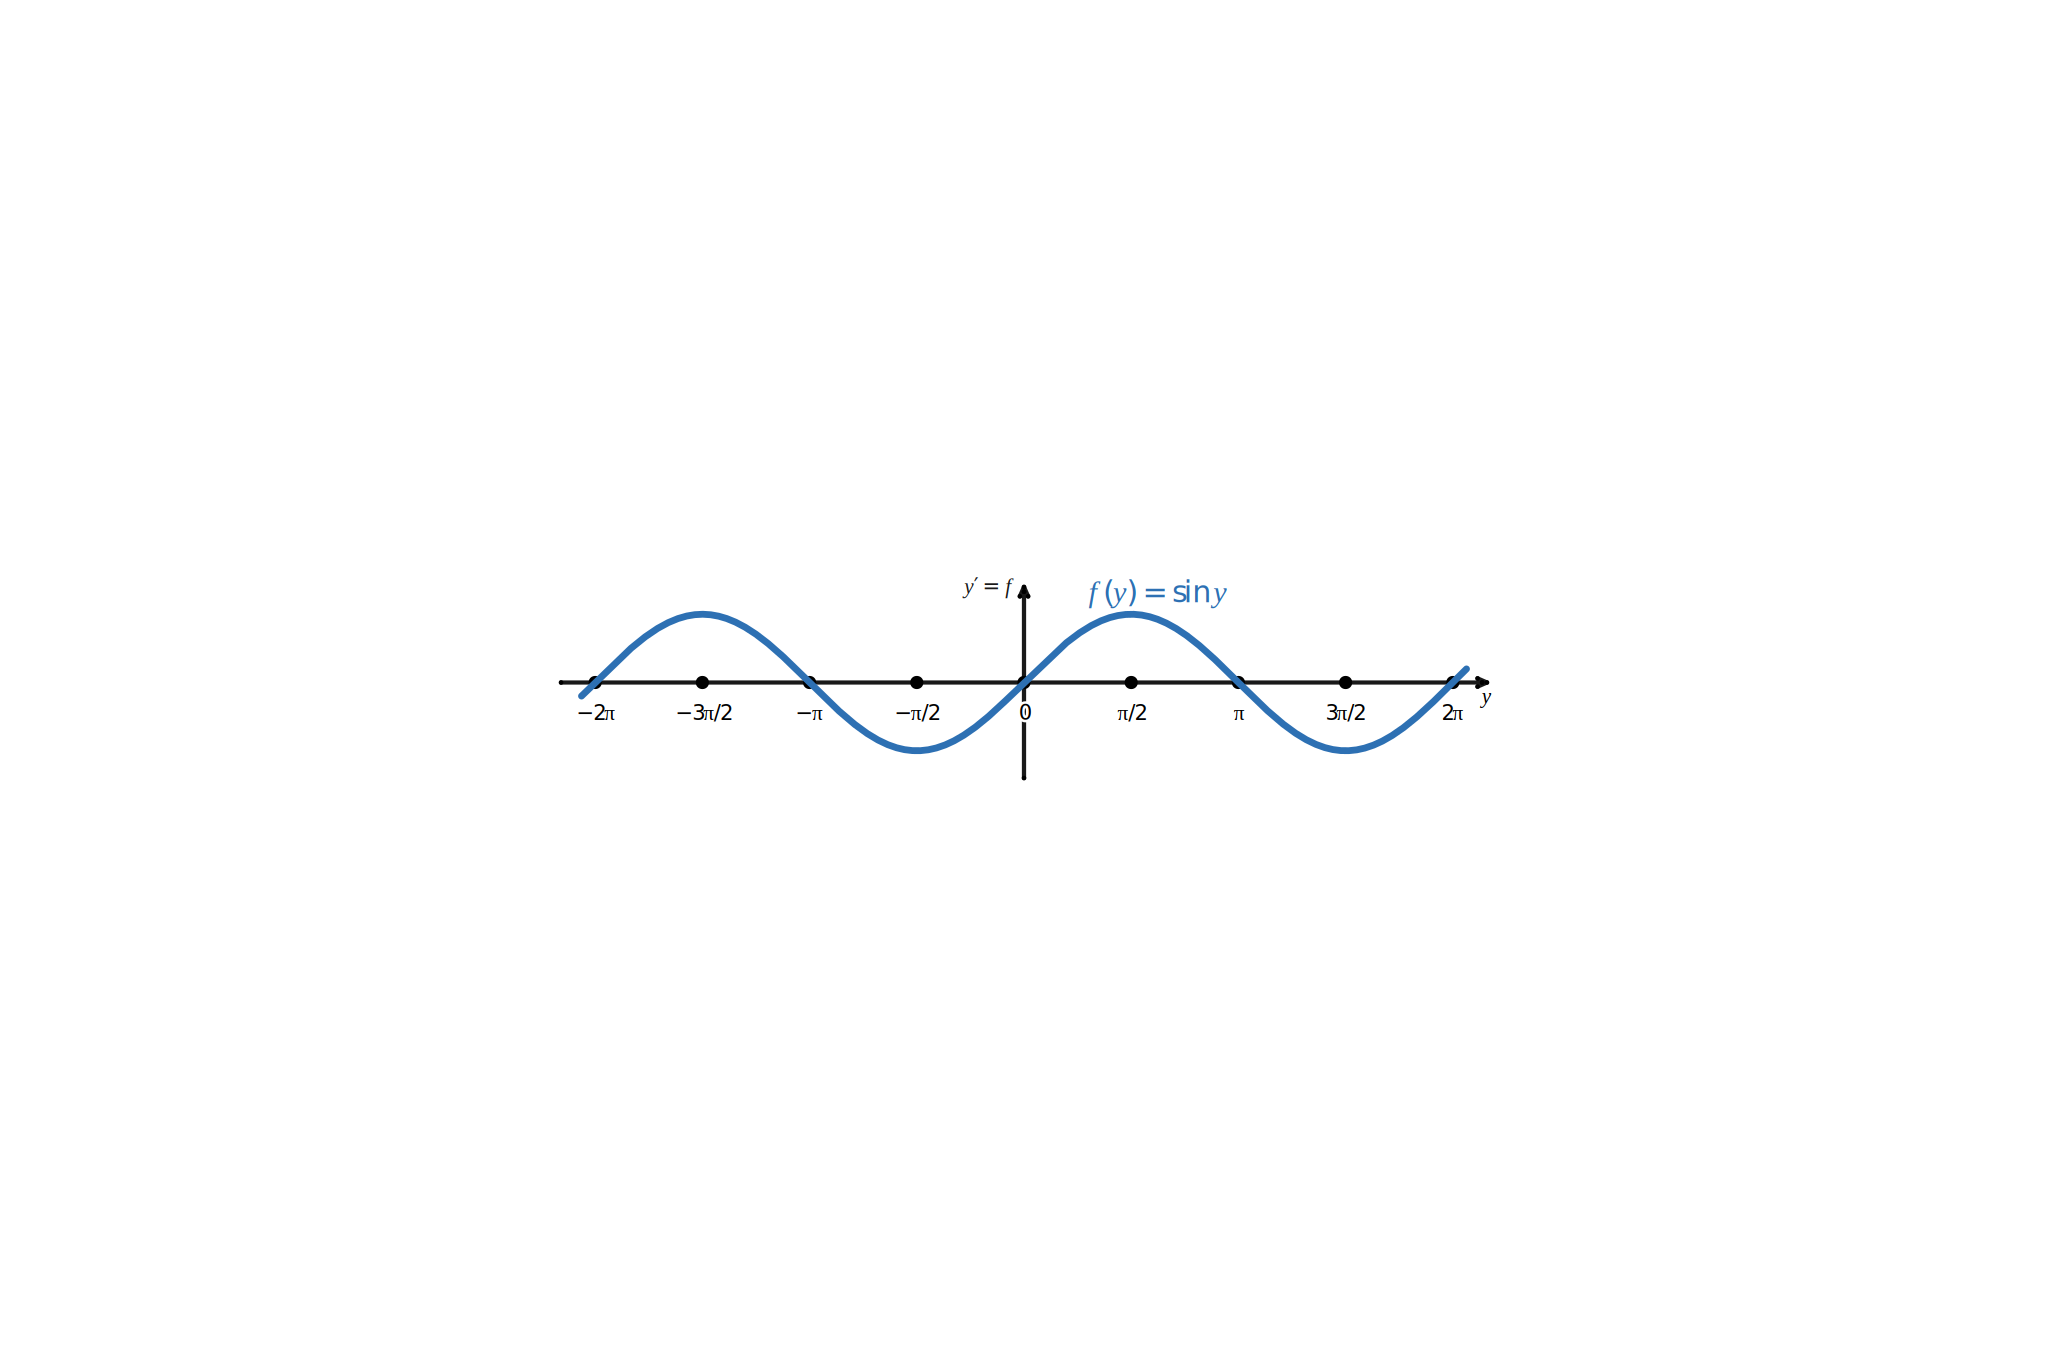
\includegraphics[width=0.9\textwidth]{additional/Stability/func.pdf}
			\caption{График в осях $y'(y)$}
		\end{figure}
		Следующим шагом определим нули производной искомой функции. Для этого необходимо приравнять правую часть $f(y)$ уравнения к нулю:
		\[ \sin{y} = 0 \implies y_n = n\pi, ~ n \in \mathbb{Z}. \]
		Для рассматриваемого случая достаточно условия, что $n = \overline{-2, 2} \subset \mathbb{Z}$. Стоит упомянуть, что для фиксированных значений $n$, $y_n$ является решением следующей задачи:
		\[ y' = \sin{y}, ~ y(0) = y_n. \]
		Такие постоянные $y_n$ называются точками покоя исходного уравнения.

		Теперь у заданной кривой определим участки, где функция $f$ положительна или отрицательна. Эти участки ограничены точками покоя. Решение $y$ уравнения $y' = f(y)$ возрастает, если $f(y) > 0$, и убывает $f(y) < 0$. Эти области пометим соответствующими направляющими стрелками:
		\begin{figure}[H]
			\centering
			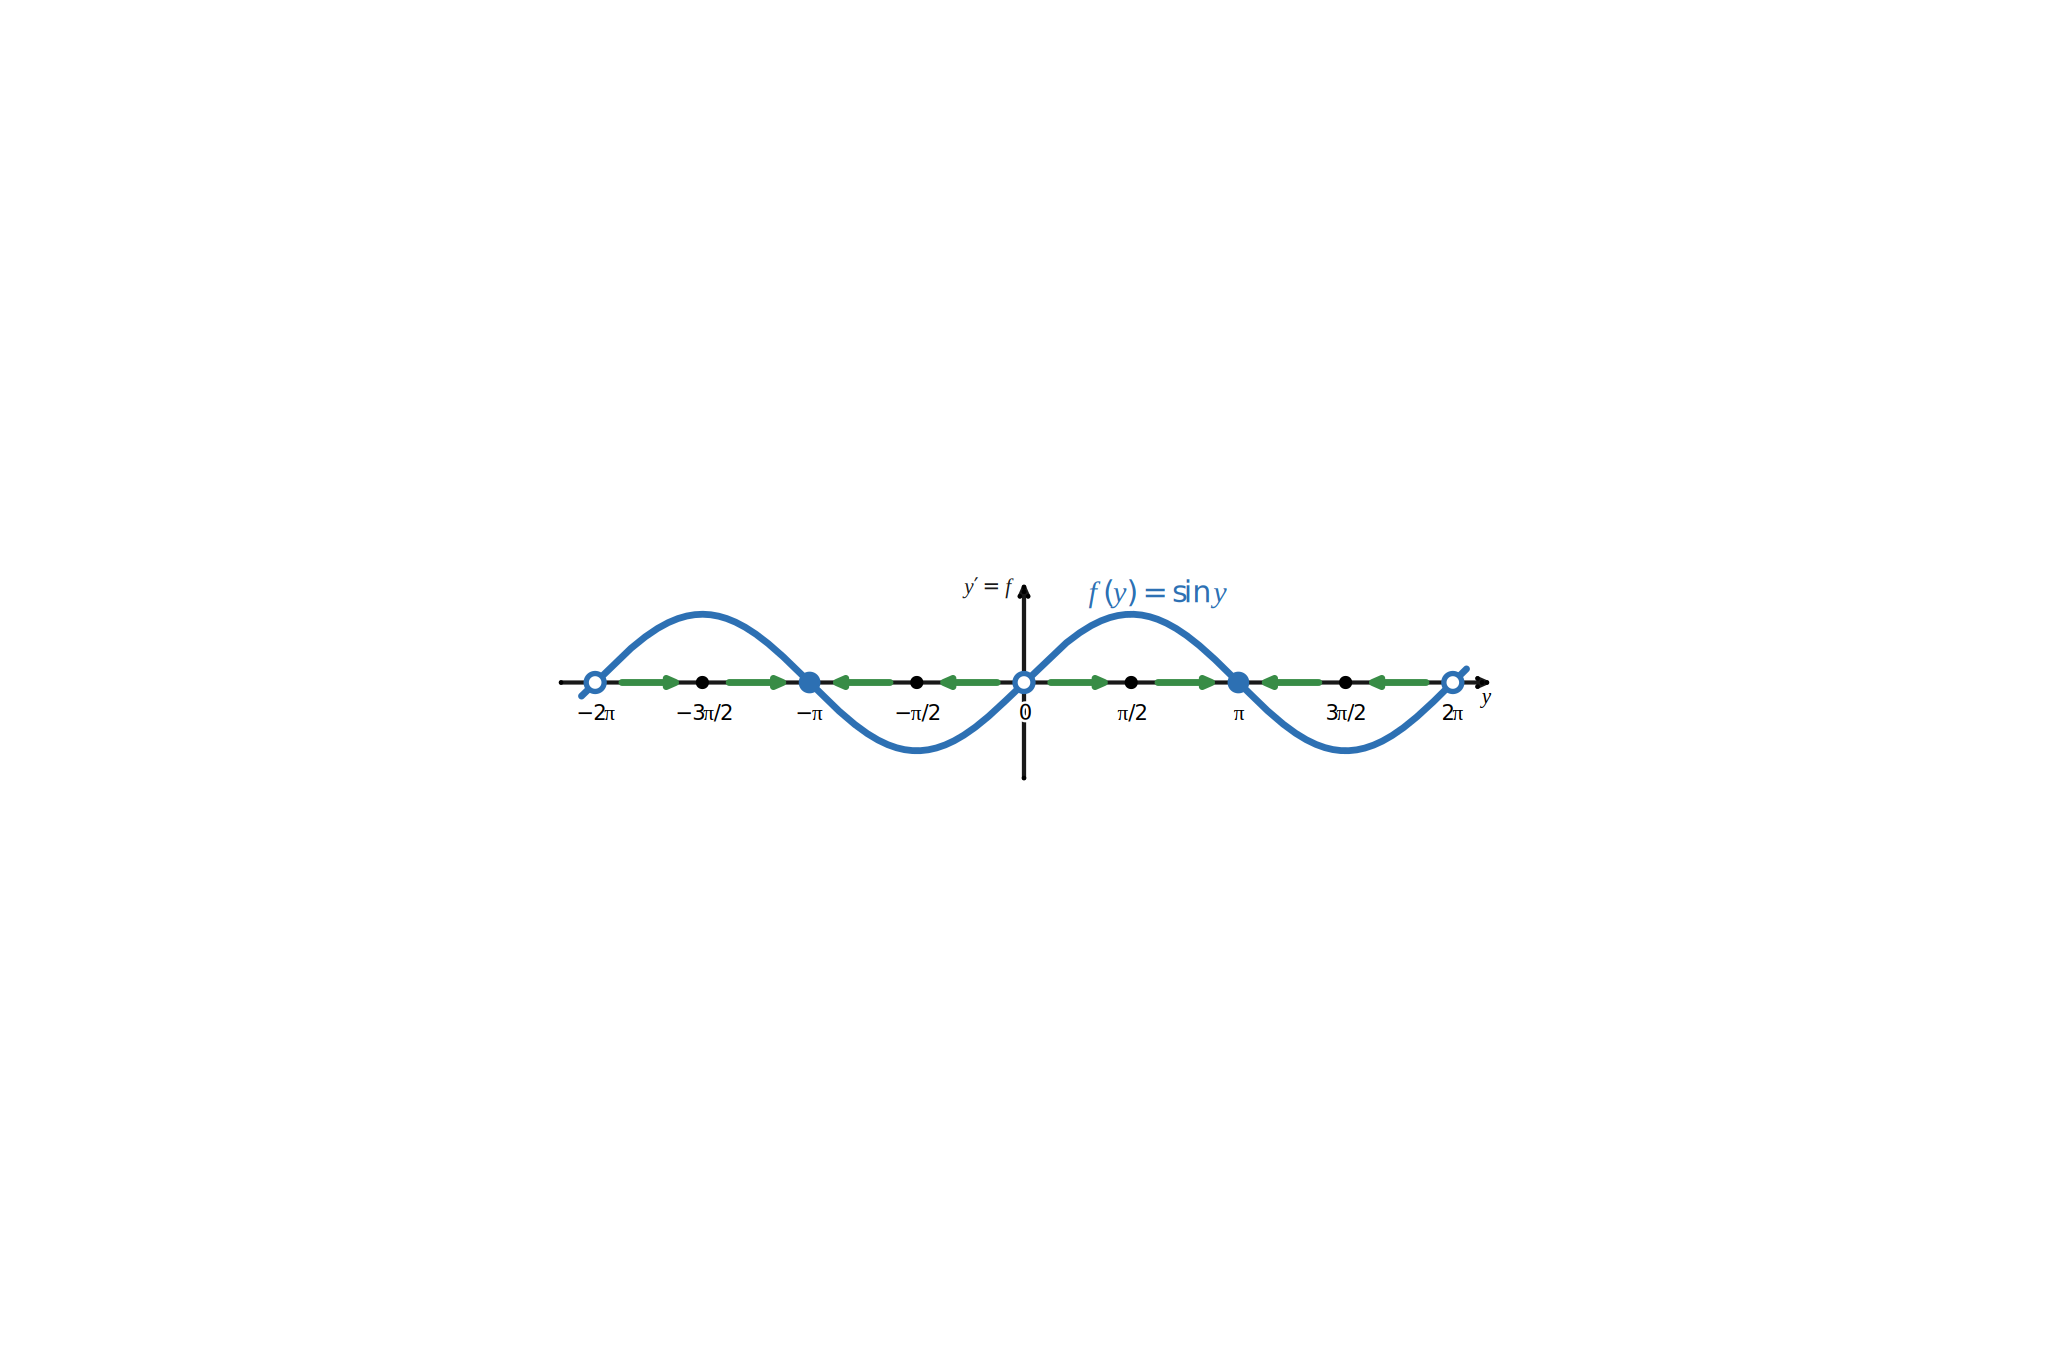
\includegraphics[width=0.9\textwidth]{additional/Stability/func_cv.pdf}
			\caption{График $f(y)$ в осях $y'(y)$ с направлениями в областях возрастания/убывания}
		\end{figure}

		Точки покоя бывают двух типов: устойчивые и неустойчивые соответственно. Согласно направляющим стрелкам, устойчивыми точками будут $y_{-1} = -\pi, ~ y_{1} = \pi$, а неустойчивыми -- $y_{-2} = -2\pi, ~ y_0 = 0, ~ y_{2} = 2\pi$. Теперь построим области перегиба кривых функции. Для этого найдем вторую производную решения:
		\[ y'' = f'(y) \cdot y' = f'(y) \cdot f(y). \]
		Области, где $y'' > 0$ -- вогнуты вверх (выпуклые), и где $y'' < 0$ -- вогнуты вниз (вогнуты).

		\pagebreak
		
		Построим график решения $f'(y)$:
		\begin{figure}[H]
			\centering
			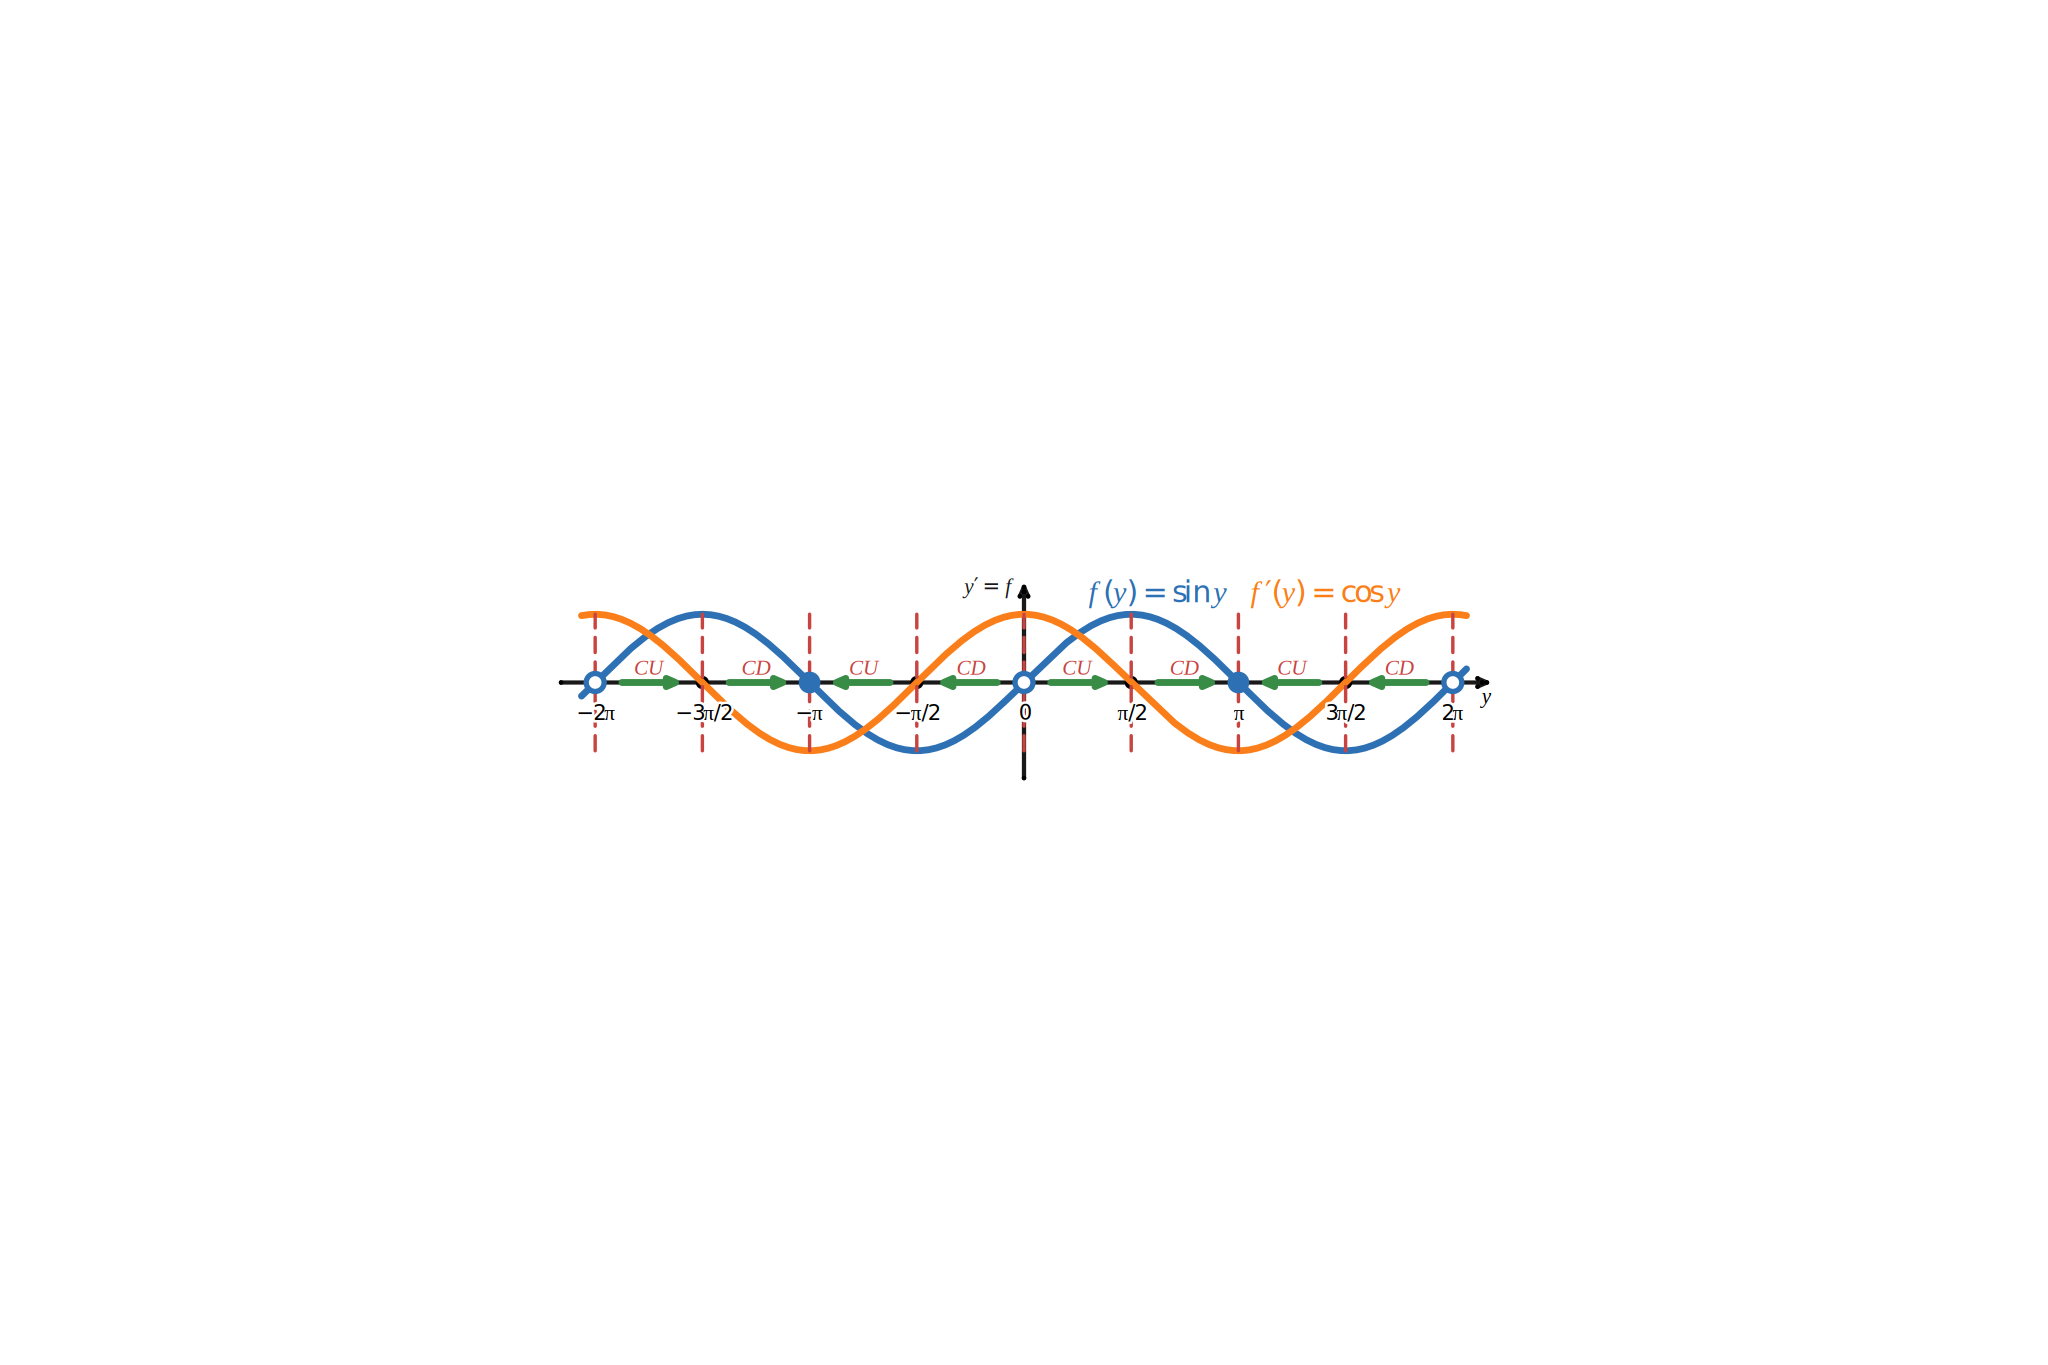
\includegraphics[width=0.9\textwidth]{additional/Stability/func_deriv_cv.pdf}
			\caption{График $f(y)$ и $f'(y)$ в осях $y'(y)$}
		\end{figure}
		На рисунке символами $CU$ и $CD$ помечены участки вогнутости вверх и вниз соответственно. Данной информации достаточно для построения примерного поведения решения исходного уравнения:
		\begin{figure}[H]
			\centering
			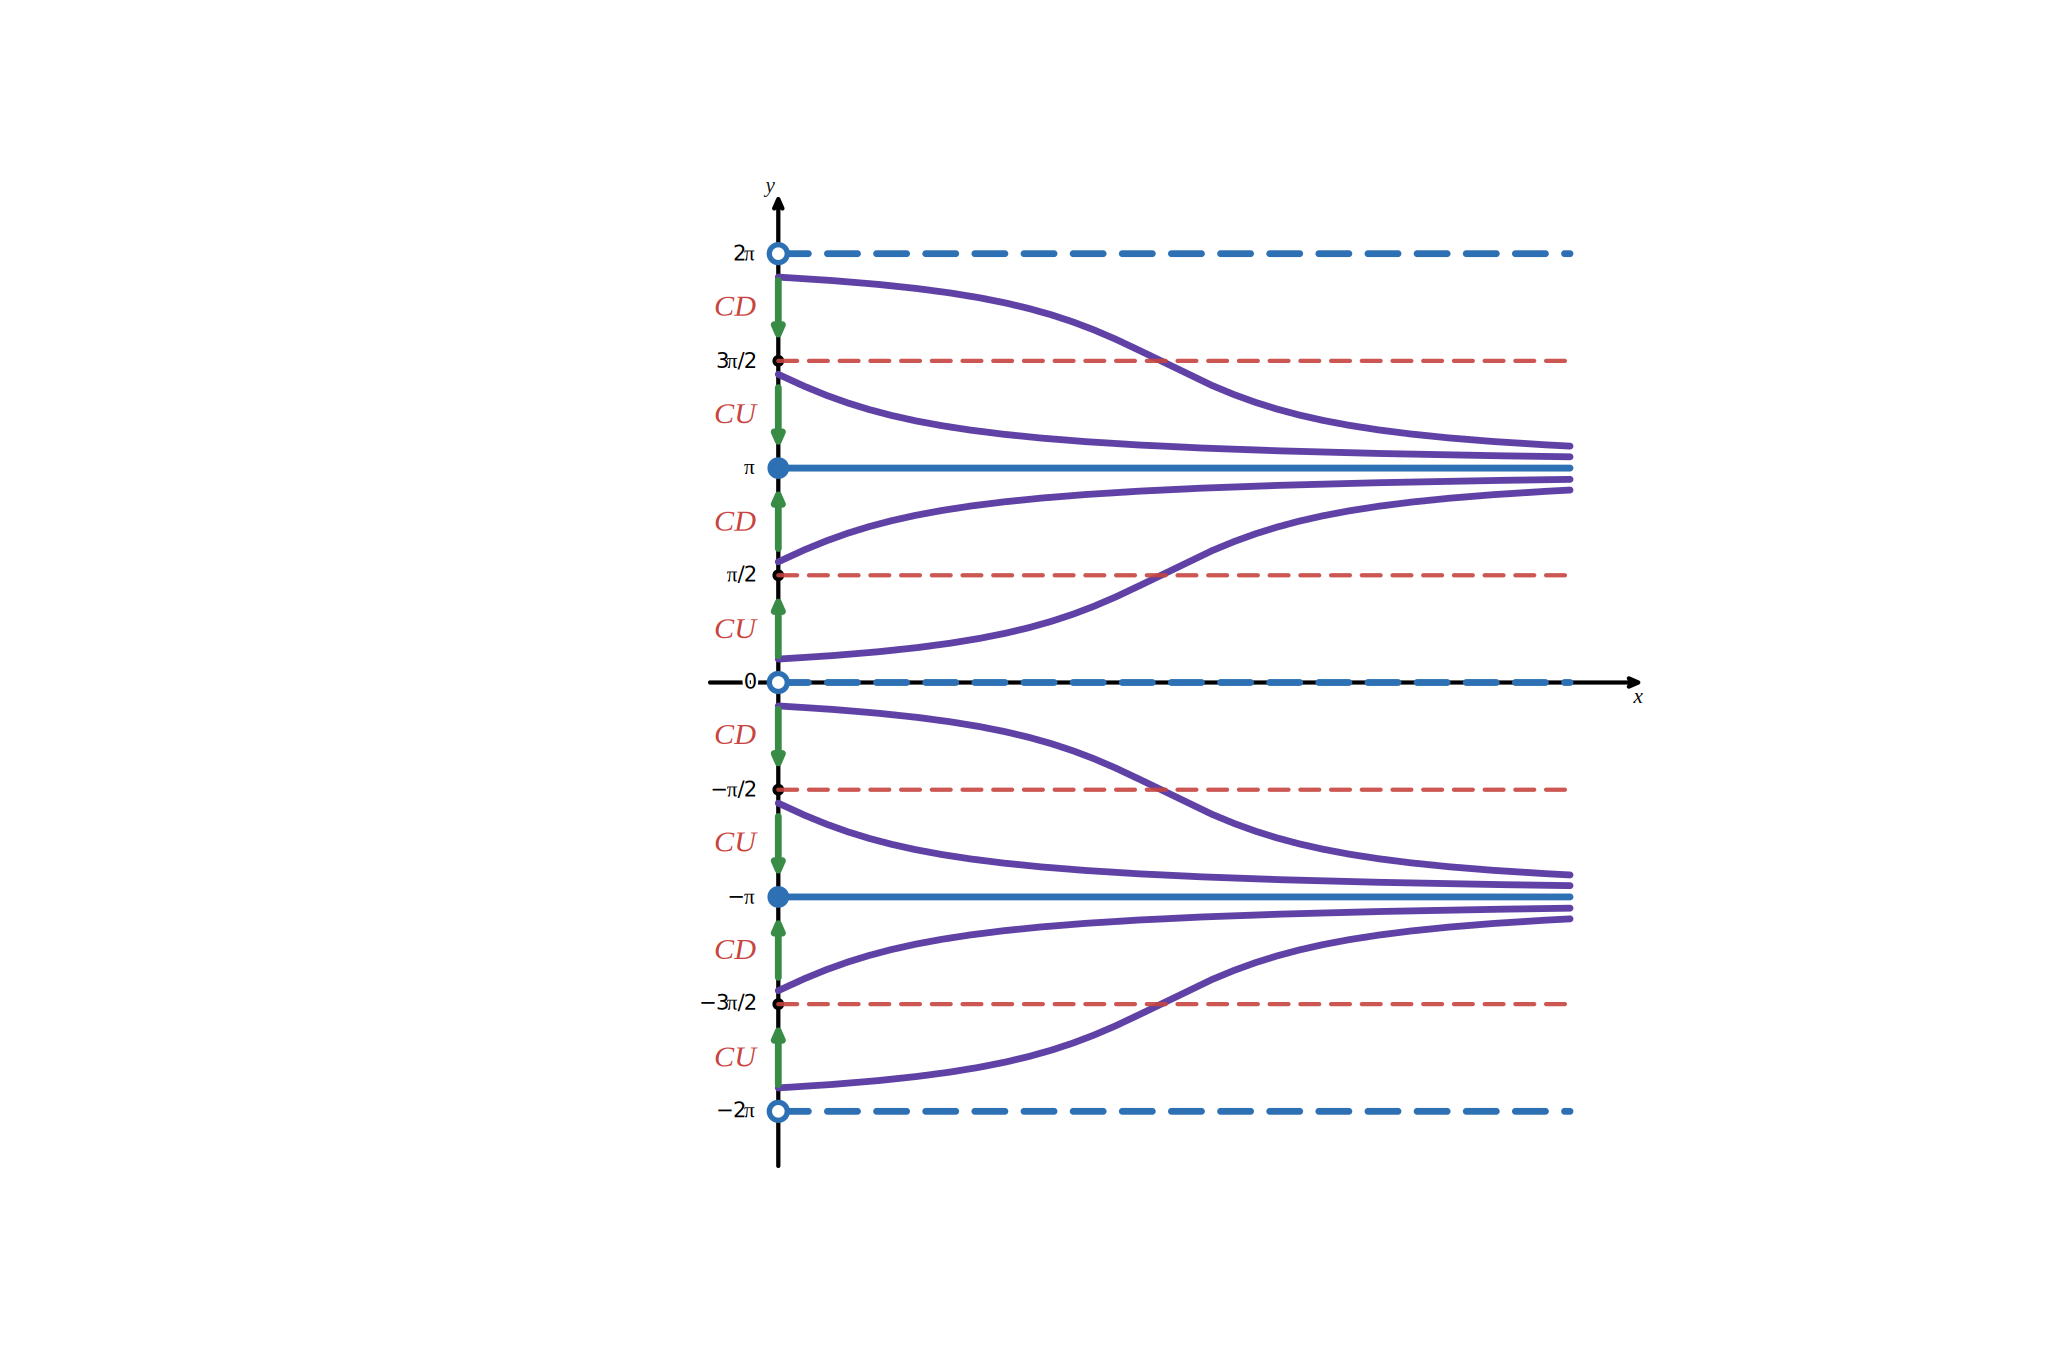
\includegraphics[width=0.8\textwidth]{additional/Stability/sols.pdf}
			\caption{Примерное поведение решения $y(x)$ исходного уравнения}
		\end{figure}

		\pagebreak

		Рассмотрим другой пример. Дана система следующего вида:
		\[ \syst{&\dot{x} = y\sin{x}, \\ &\dot{y} = x\sin{y}}. \]
		Необходимо найти точки покоя, и исследовать их устойчивость. Найдем все возможные точки покоя. Для этого приравняем производные к нулю:
		\[ \syst{&\dot{x} = 0, \\ &\dot{y} = 0.} \implies \syst{&y \sin{x} = 0, \\ &x \sin{y} = 0.} \]
		Из этой системы следует набор таких точек:
		\[ \syst{&x = n\pi, \\ &y = m\pi.}, ~ n, m \in \mathbb{Z} \]
		Построим матрицу Якоби исходной системы в окрестности точки $\pares{n\pi, m\pi}$:
		\[ A = J\pares{x, y} \at_{\pares{n \pi, m \pi}} = \begin{pmatrix} 
			\dpart{}{x}\pares{y \sin{x}} & \dpart{}{y}\pares{y \sin{x}} \\
			\dpart{}{x}\pares{x \sin{y}} & \dpart{}{y}\pares{x \sin{y}}
		\end{pmatrix} \at_{\pares{n \pi, m \pi}} = \begin{pmatrix}
			(-1)^n m \pi & 0 \\
			0 & (-1)^m n \pi
		\end{pmatrix}. \]
		Найдем собственные значения данной матрицы:
		\[ \det{\abs{A - \lambda I}} = 0 \implies \bpares{\lambda - (-1)^n m \pi} \cdot \bpares{\lambda - (-1)^m n \pi} = 0. \]
		Отсюда следует, что $\lambda_1 = (-1)^n m \pi$ и $\lambda_2 = (-1)^m n \pi$. 

		Рассмотрим случаи, когда собственные значения отрицательны одновременно:
		\begin{enumerate}
			\item $n > 0, m > 0$: Если $n$ и $m$ нечетные одновременно;
			\item $n < 0, m < 0$: Если $n$ и $m$ четные одновременно;
			\item $n < 0, m > 0$: Если $n$ -- нечетное, $m$ -- четное;
			\item $n > 0, m < 0$: Если $n$ -- четное, $m$ -- нечетное.
		\end{enumerate}
		Случаи, содержащие $m = 0$, или $n = 0$ не рассматриваем, так как их исследование на устойчивость требует дополнительного анализа. Все остальные случаи сводятся к наличию хотя бы одного положительного собственного значения, что говорит о том, что система не устойчива. В общем случае здесь можно заметить некоторую симметрию относительно $n$ и $m$.

	% \pagebreak